\documentclass[border=10pt]{standalone}
\usepackage{pgfplots}
\pgfplotsset{compat=1.17}

\begin{document}
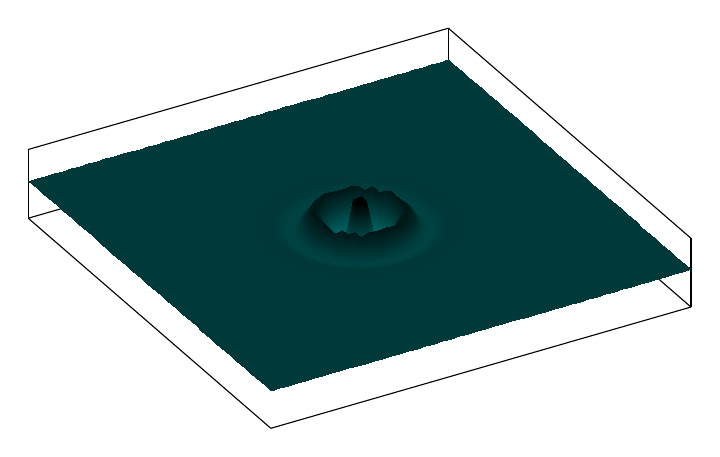
\begin{tikzpicture}
    \begin{axis}[
        view={60}{30},
        axis lines=box,
        axis equal image,
        width=10cm,
        height=10cm,
        xlabel={},
        ylabel={},
        zlabel={},
        xtick=\empty,
        ytick=\empty,
        ztick=\empty,
        colormap={teal}{color=(teal) color=(black)},
        shader=interp,
        domain=-5:5,
        y domain=-5:5,
        samples=50,
        z buffer=sort
    ]
        \addplot3[surf] {exp(-x^2-y^2)*cos(deg(2*pi*sqrt(x^2+y^2)))};
    \end{axis}
\end{tikzpicture}
\end{document}